\section{Paths and Connectivity}
Graphs are similar to train networks or airline routes. They connect one 
location to another.

\begin{Def}[Graph]

    A \textbf{graph} is a collection of points, called \textbf{vertices} or \textbf{nodes}, 
    connected by lines, called \textbf{edges}. Similarly to how a polygon has vertices connected by edges.

\end{Def}
\begin{Def}[Undirected Graph]

    An \textbf{undirected graph} is a graph where the edges have no particular direction going both ways between nodes. 
    A \textbf{degree} of a node is the number of edges connected to it.
\end{Def}
\noindent
\textbf{Example:} Figure (\ref{fig:undir_graph}) shows an undirected graph:\\
\begin{figure}[h]
    \begin{center}
      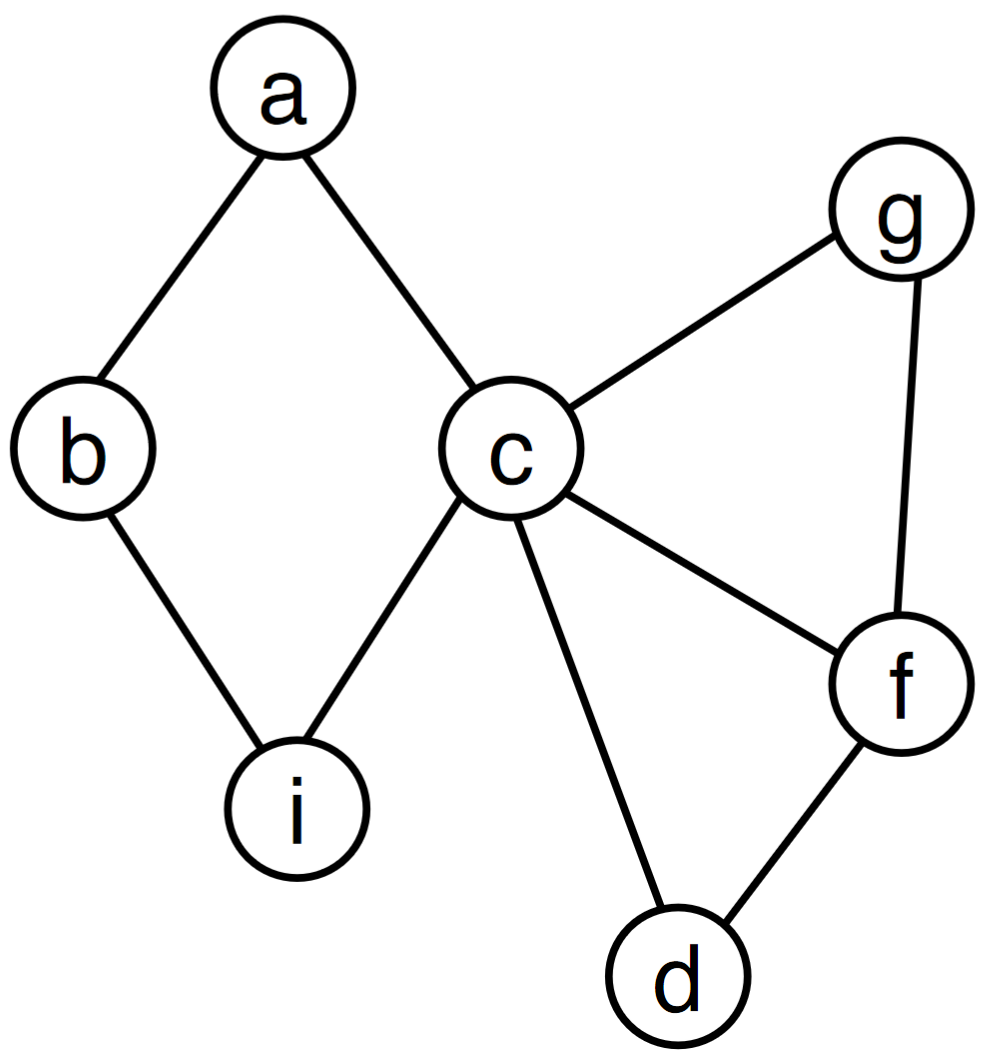
\includegraphics[height=1.8in]{./Sections/graphs/undir_graph.png}
    \end{center}
     \caption{An undirected graph with 7 vertices and 9 edges.}\label{fig:undir_graph}
  \end{figure}

\noindent
Node $a$ has a degree of 3, and node $c$ has a degree of 4.\\
\newpage

\begin{Def}[Directed Graph]

    A \textbf{directed graph} is where the edges have a specific direction from one node to another.
    \begin{itemize}
        \item  The \textbf{indegree} of a node is the number of edges that point to it.
        \item The \textbf{outdegree} of a node is the number of edges that point from it.
    \end{itemize}
\end{Def}
\noindent
\textbf{Example:} Figure (\ref{fig:dir_graph}) shows a directed graph:\\
\begin{figure}[h]
    \begin{center}
      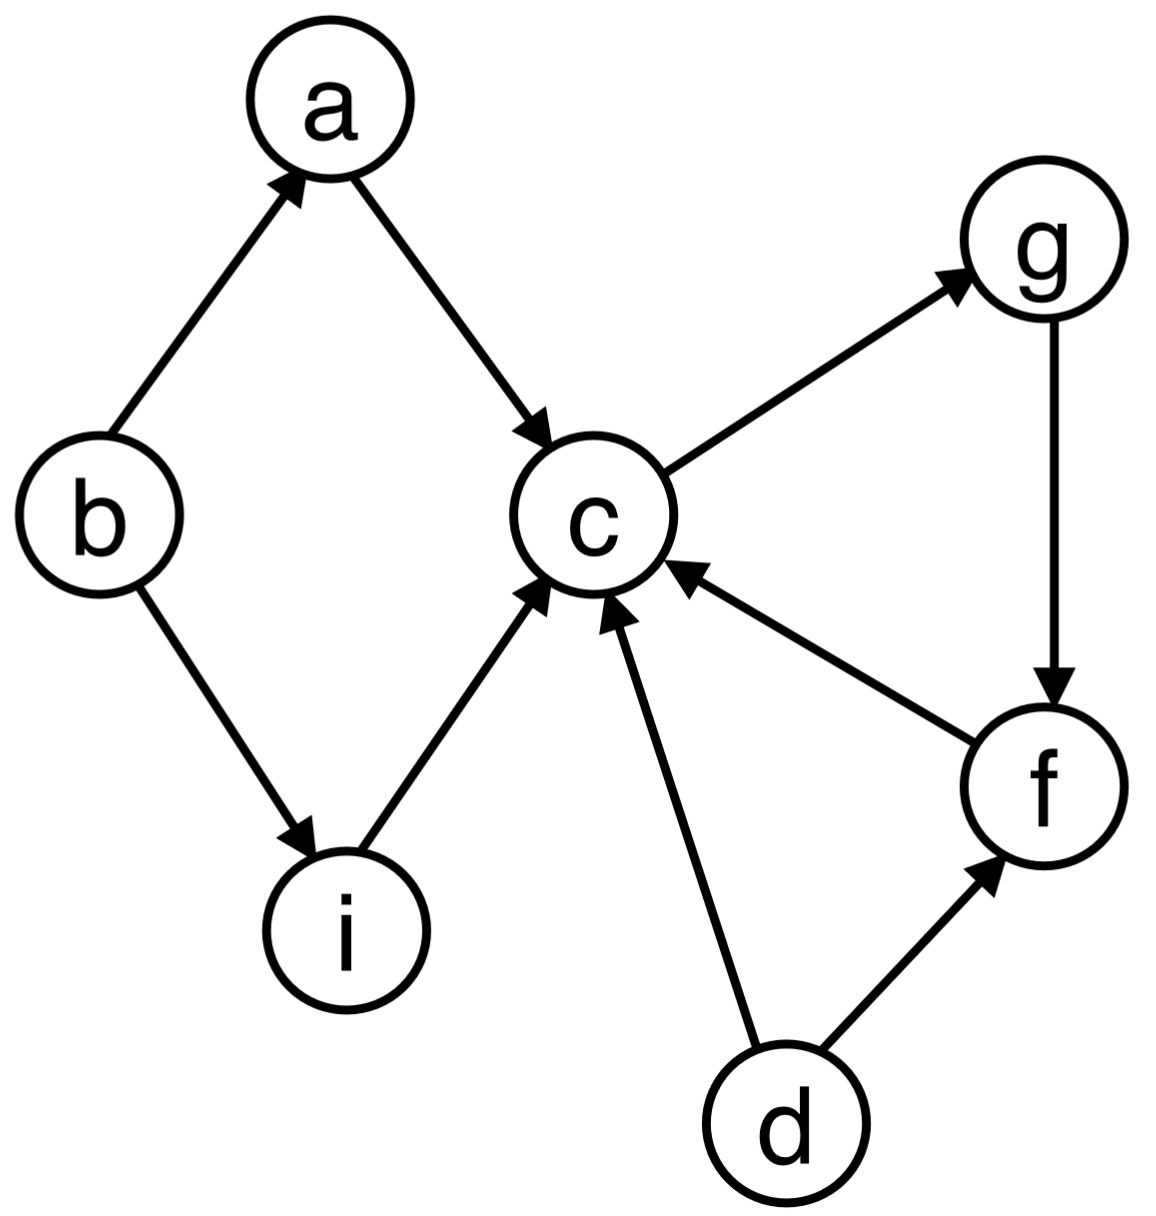
\includegraphics[height=1.5in]{./Sections/graphs/dir_graph.png}
    \end{center}
     \caption{A directed graph with 7 vertices and 9 edges.}\label{fig:dir_graph}
  \end{figure}

  \noindent
    Node $b$ has an outdegree of 2 and an indegree of 0. $c$ has an indegree of 4 and an outdegree of 0.

\begin{Def}[Weighted Graph]

    A \textbf{weighted graph} is a graph where each edge has a numerical value assigned to it.
\end{Def}
\noindent
\textbf{Example:} Figure (\ref{fig:weight_graph}) shows a weighted graph:\\
\begin{figure}[h]
    \begin{center}
      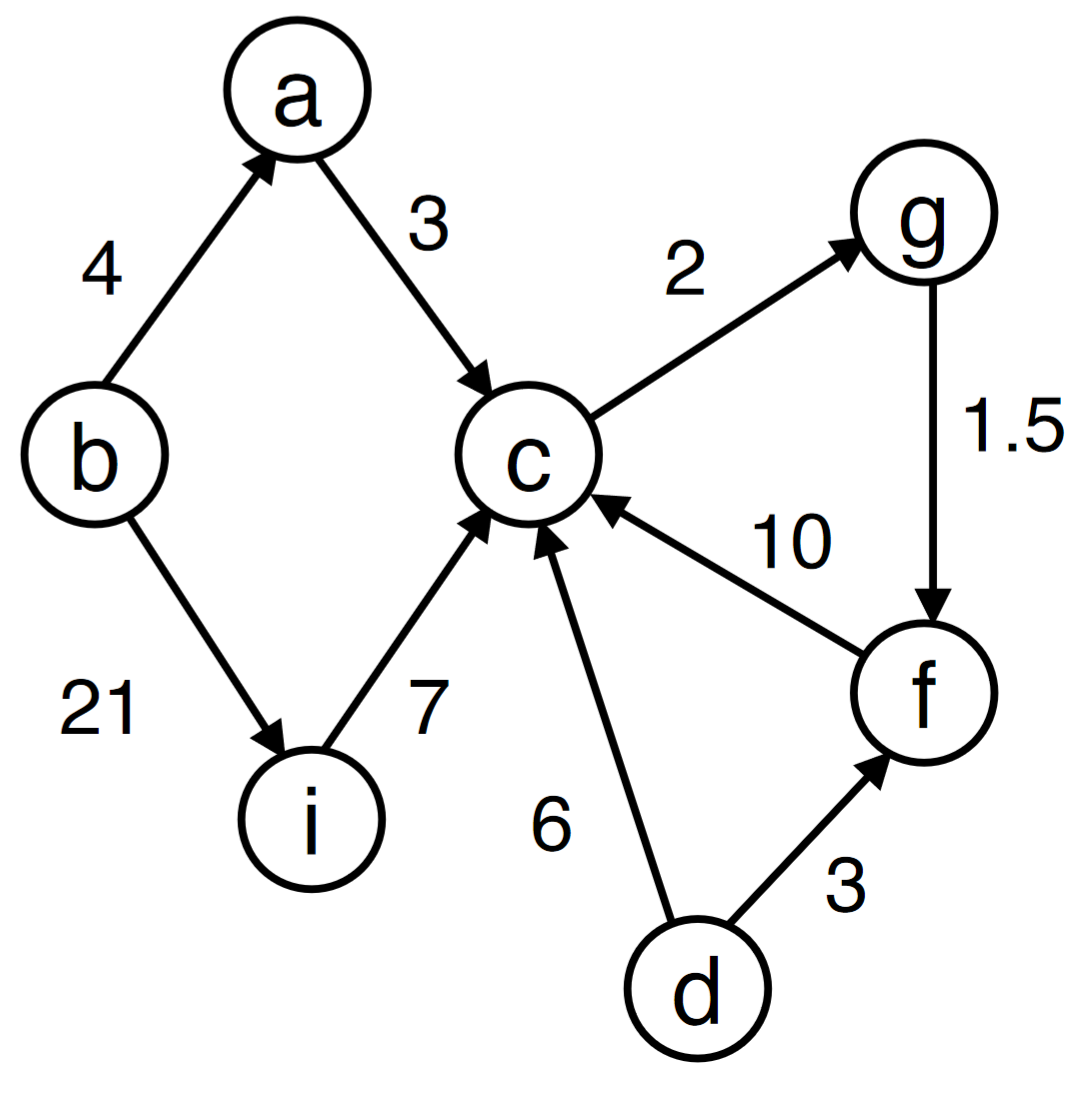
\includegraphics[height=1.5in]{./Sections/graphs/weight_graph.png}
    \end{center}
     \caption{A weighted graph with 7 vertices and 9 edges.}\label{fig:weight_graph}
  \end{figure}
\newpage
\begin{Def}[Path]

    A \textbf{path} is a sequence of edges that connect a sequence of vertices. A 
    path is \textbf{simple} if all nodes are distinct.
\end{Def}

\noindent
\textbf{Example:} In Figure (\ref{fig:path_graph}), a simple path $h\leftrightarrow b \leftrightarrow i \leftrightarrow c \leftrightarrow d$ is shown:\\
\begin{figure}[h]
    \begin{center}
      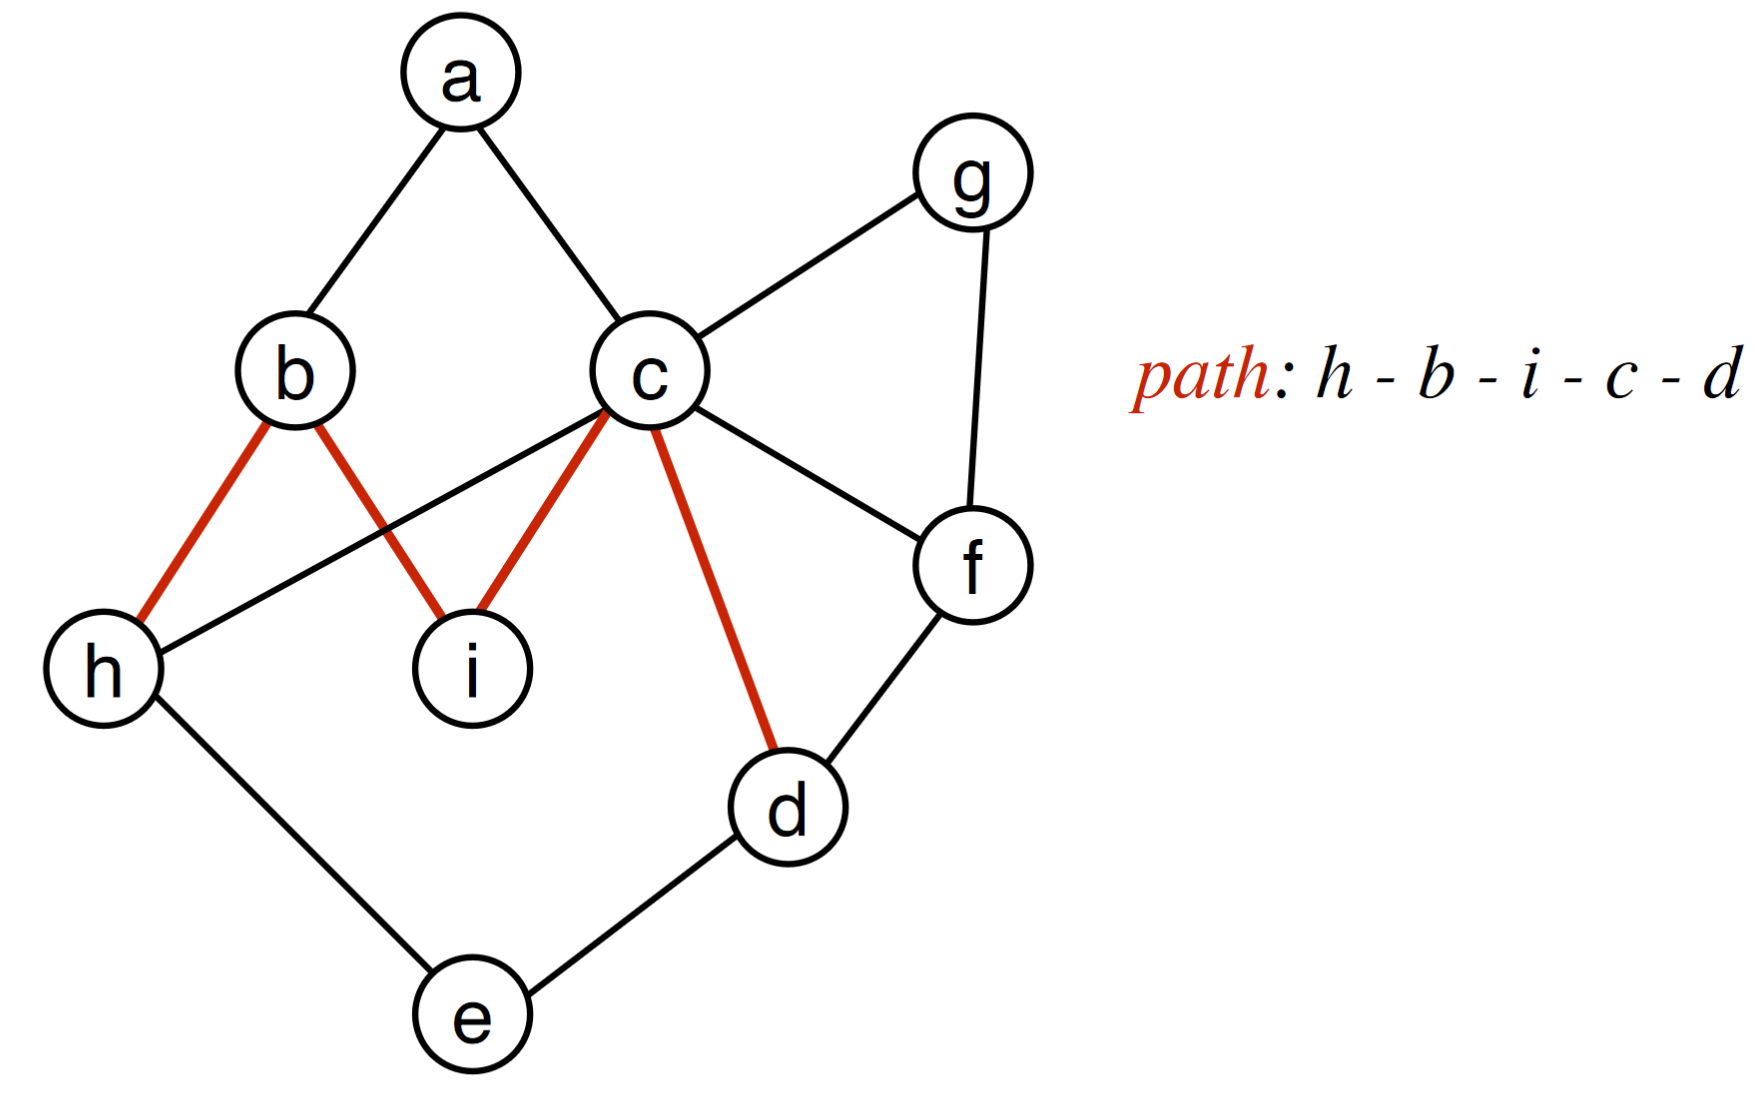
\includegraphics[height=1.8in]{./Sections/graphs/path_graph.png}
    \end{center}
     \caption{A graph with a simple path from $h$ to $d$.}\label{fig:path_graph}
  \end{figure}

\begin{Def}[Connectivity]

    A graph is \textbf{connected} if there is a path between every pair of vertices. 
    A graph is \textbf{disconnected} if there are two vertices with no path between them.
\end{Def}
\textbf{Example:} In Figure (\ref{fig:con_graph}), shows connected and disconnected graphs:\\
\begin{figure}[h]
    \begin{center}
      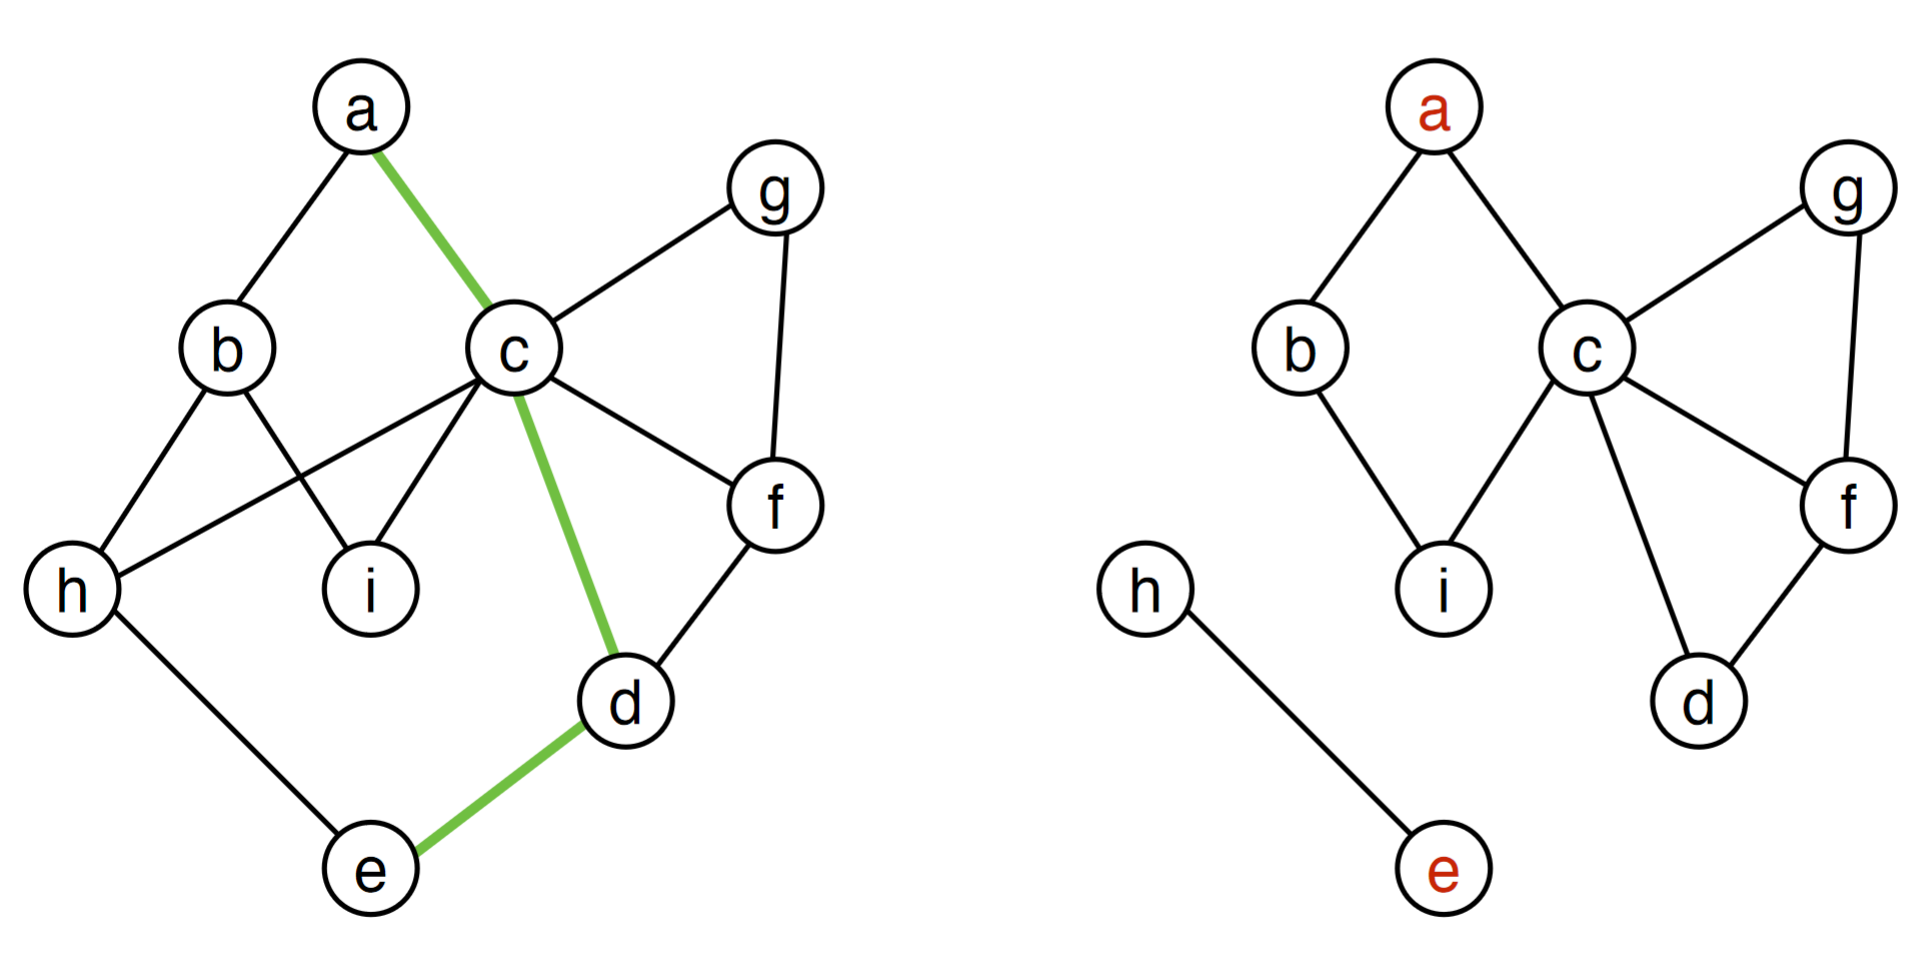
\includegraphics[height=1.8in]{./Sections/graphs/con_graph.png}
    \end{center}
     \caption{A connected graph $a\leftrightarrow c \leftrightarrow d \leftrightarrow e$  and disconnected graph.}\label{fig:con_graph}
  \end{figure}
  



